\documentclass{article}
\usepackage{graphicx} % Required for inserting images
\usepackage[dvipsnames]{xcolor}
\usepackage[margin=2.5cm]{geometry} %Au lieu de 1.5cm ? Tu aimes mieux comme ça mon chouchou (anciennement 2.5cm)?
\usepackage{hyperref}
\hypersetup{
    colorlinks=true,
    urlcolor=blue,
    linkcolor=blue,
    breaklinks=true
}

\title{Gestion de Projet Informatique}
\author{ALBRECHT Maël - HAMMOUDA Rayane\\MAISONNETTE Elouan - RICARD Noah}
\date{Mars 2026}

\begin{document}

\maketitle

%%%%%%%%%%%%%%%%%%%% %%%%%%%%%%%%%%%%%%%% %%%%%%%%%%%%%%%%%%%%

\section*{\color{Green}[A1] Constitution d'un groupe} %ajout d'une étoile après "section" pour retirer la numérotation automatique
Suite aux cours de Gestion de projet professionnel auprès du prof Bertrand Kerautret, un mini-projet doit être réalisé, afin de montrer l'acquisition des compétences liées au logiciel de gestion de versions Git.\break

Maël ALBRECHT, Rayane HAMMOUDA, Elouan MAISONNETTE et Noah RICARD se sont organisés au sein du groupe de TD003, pour réaliser une page web sur un sujet de culture populaire dans le cadre de ce projet. Noah R. s'occupe de mettre à jour le dépôt, Elouan M. se charge de l'avancée du compte rendu \LaTeX, tandis que Rayane H. et Maël A. s'occupent de la partie JavaScript et CSS du site ; tout le monde participe à la structure du code HTML.

\begin{center}
    Pseudonymes GitHub : \href{https://github.com/Alem154}{Alem154} - \href{https://github.com/rayanehammouda89-beep}{rayanehammouda89-beep} - \href{https://github.com/Eloulan}{Eloulan} - \href{https://github.com/Mushi-027}{Mushi-027}

    Nous faisons tous les quatre partie de l'organisation \href{https://github.com/GestProjTD3-HARM}{GestProjTD3-HARM} (\ref{fig:mb-orga-GH}).
\end{center}

\begin{figure}[ht]  %Figure est un float en passant les options h -here- et t -top- vous forcer (grace au h) l'image à l'endroit le plus haut (le t) depuis sa mention autre option [b] (bottom) et [p] (p = separate page)
    \centering
    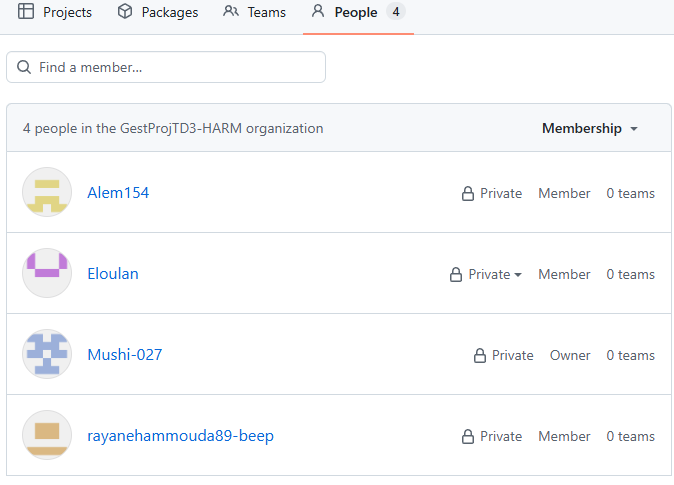
\includegraphics[width=0.5\linewidth]{Equipe.png}
    \caption{Capture d'écran des membres de l'organisation}
    \label{fig:mb-orga-GH}
\end{figure}

%%%%%%%%%%%%%%%%%%%% %%%%%%%%%%%%%%%%%%%% %%%%%%%%%%%%%%%%%%%%

\section*{\color{Green}[A2] Dépôt Git en ligne}
Lien du dépôt en ligne : \url{https://github.com/GestProjTD3-HARM/ProjetFinal-GestProj}
\newpage
\begin{figure}[ht]
    \centering
    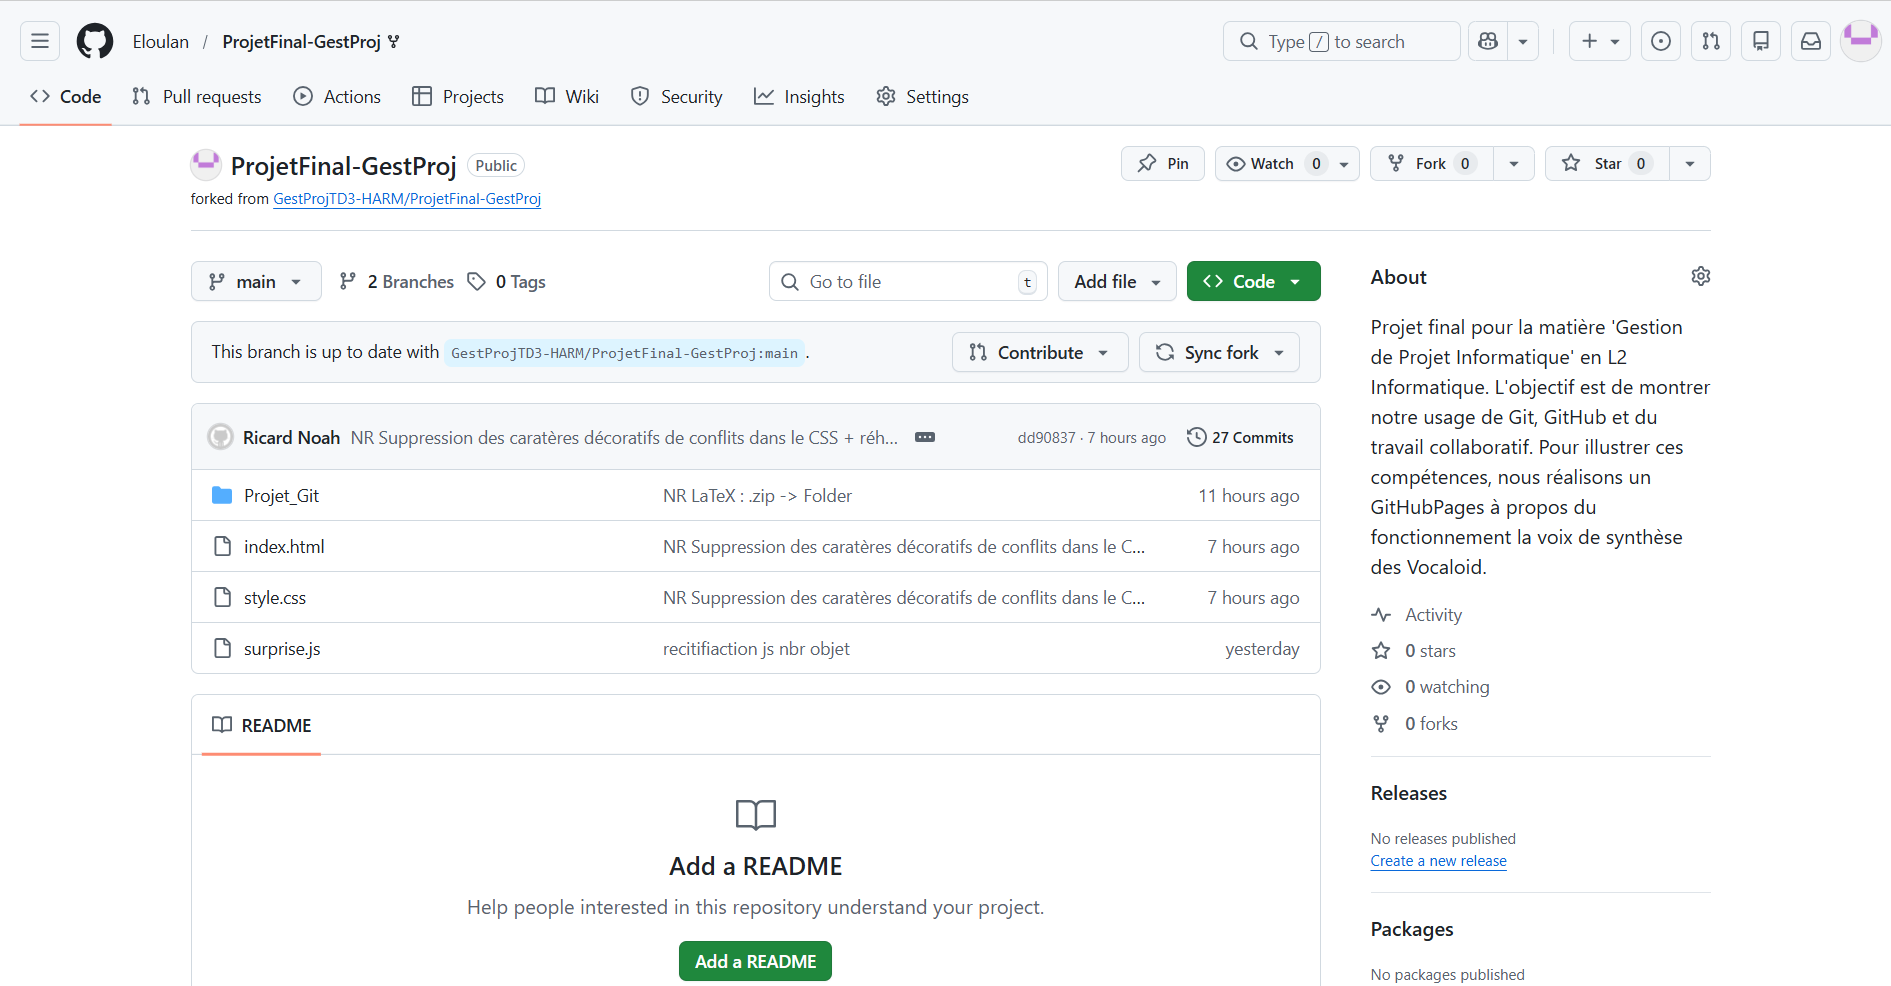
\includegraphics[width=0.7\textwidth]{Repository.png}
    \caption{Le dépôt du mini-projet}
\end{figure}
Grâce à ce dépôt l'équipe peut facilement échanger leurs ajouts de façon pratique et immédiate... %Restitution du cours
\\Les étapes suivantes seront plus orientées vers la construction d'un environnement GitHub profitant d'un maximum de ces fonctions

%%%%%%%%%%%%%%%%%%%% %%%%%%%%%%%%%%%%%%%% %%%%%%%%%%%%%%%%%%%%

\section*{\color{Green}[A3] Intégration des contributions}
Les premiers commits, n'ayant pas encore à ce moment associés tout le monde en collaborateurs, ont un nom différent lors des commits (\ref{fig:first-commits}). %Desolé Noah enfaite c'est moi qui commit avec DES ordis différents (celui du cours, celui de chez moi, une session pour chaque ordi de la salle info) --- tkt, j'ai fait la même :') 'Noah'

Chaque membre peut \textit{push} de leur côté et après vérification de la part des autres, être affecté au projet final.
\begin{figure}[ht]
    \centering
    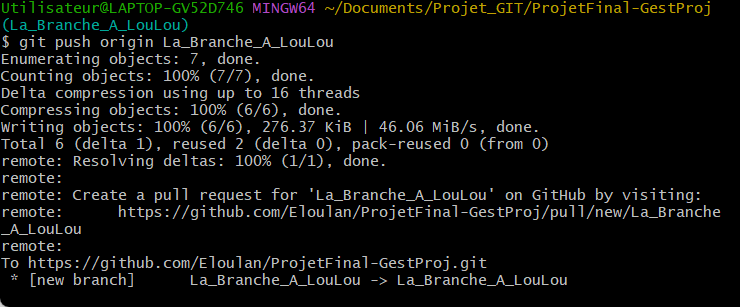
\includegraphics[width=0.5\linewidth]{PushCommand.png}
    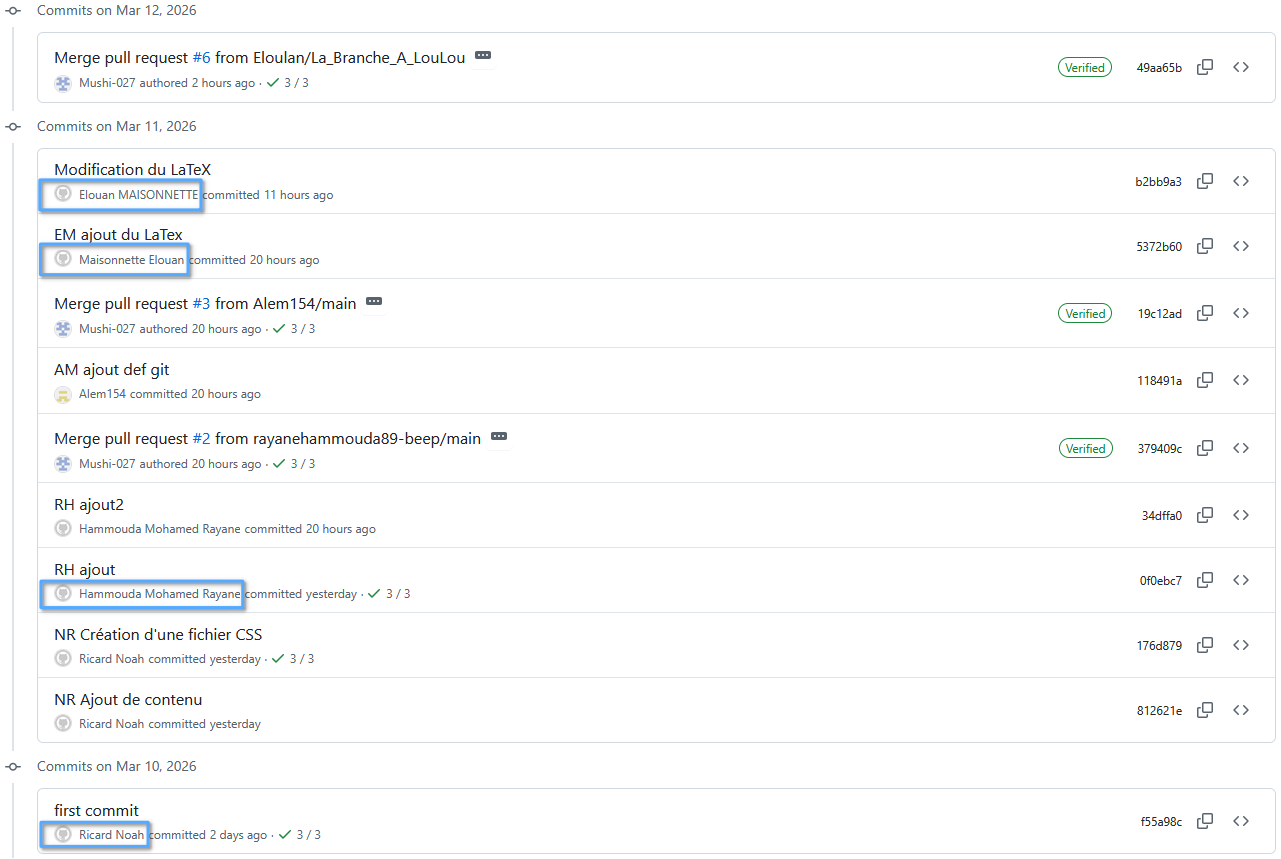
\includegraphics[width=0.5\linewidth]{First-commits.png}
    \caption{Captures d'écran d'un \textit{push} vers le dépôt et des premiers commits \textit{push} vers le projet principal}
    \label{fig:first-commits}
\end{figure}

%%%%%%%%%%%%%%%%%%%% %%%%%%%%%%%%%%%%%%%% %%%%%%%%%%%%%%%%%%%%

\section*{\color{BurntOrange}[B1] Gestion par branches}
Des branches furent créées afin de faire des tests avant l'ajout à la branche principale \textit{main}, notamment pour faire des tests sur le document \LaTeX afin de pouvoir modifier le document collaborativement avant implémentation dans la branche finale. 
%Je m'apprête à créer une branche pour cette version car les marges du LaTeX m'ont été proposée à 1.5cm mais je pense que 2.5cm pourrait être mieux. Pourquoi pas un entre deux, le LaTeX devra être restructuré dans le cas d'un changement de marge avant qu'un 'merge' soit fait avec la branche principale.
\begin{figure}[ht]
    \centering
    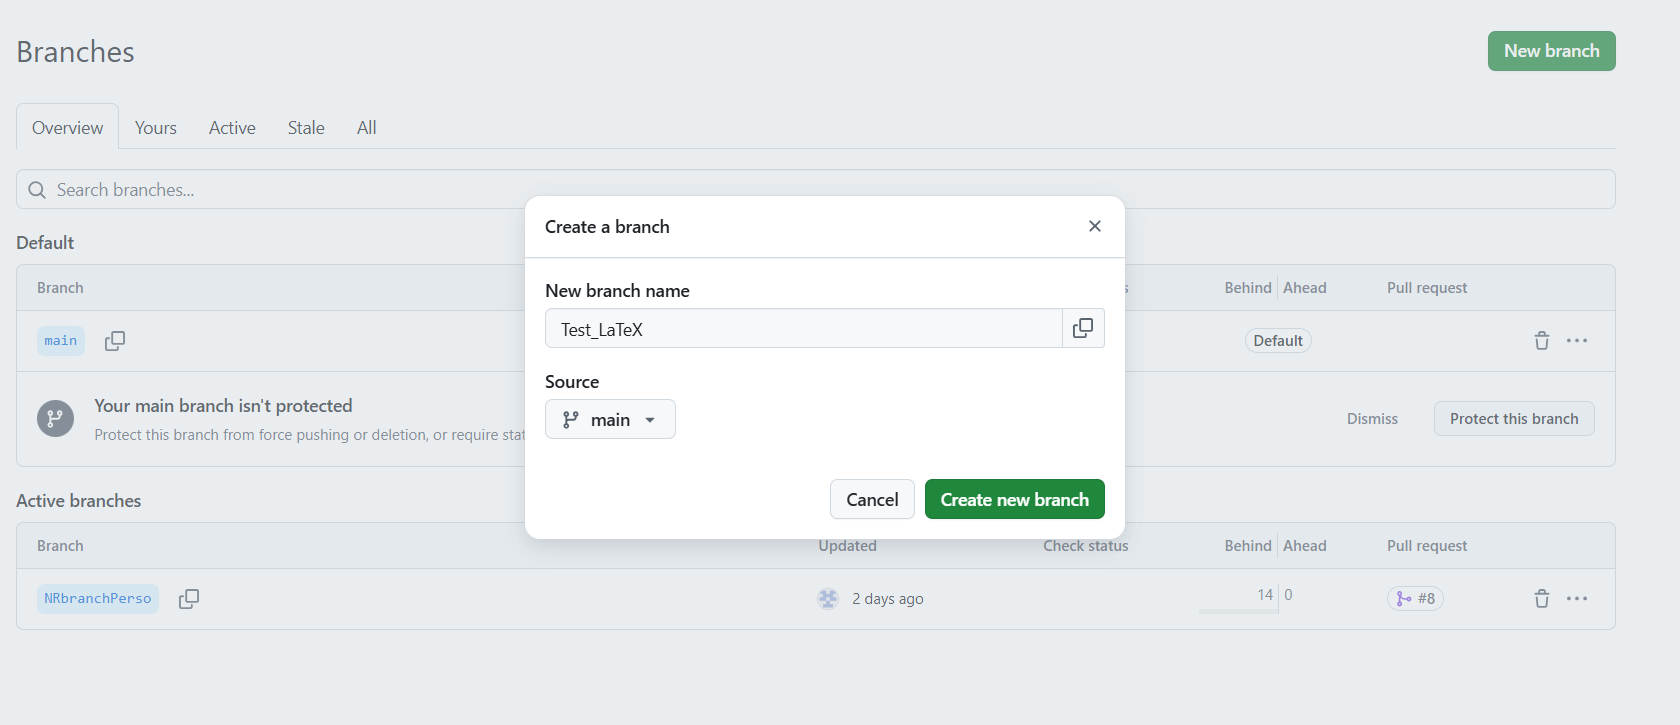
\includegraphics[width=0.7\linewidth]{CréationBranch.png}
    \caption{Création d'une branche pour les changements du \LaTeX}
    \label{fig:branch_latex}
\end{figure}

%%%%%%%%%%%%%%%%%%%% %%%%%%%%%%%%%%%%%%%% %%%%%%%%%%%%%%%%%%%%

\section*{\color{BurntOrange}[B2] Intégration de version et tag}
Les tags permettent une navigation simplifiée par la création de versions qui marquent les étapes majeures dans l'évolution du projet, les versions donnent un titre plus officiel au commit auquel le tag est associé, en utilisant la commande:

\begin{center}
    \textbf{git tag -a v1.0 -m "première version"}
\end{center}

Grâce à cette commande, on officialise une première version de notre site, que l'on peut annoter avec l'option "-a V1.0" qui enregistre la date et l'auteur du tag, ainsi que le message renseigné après "-m message"
\begin{figure}[ht]
    \centering
    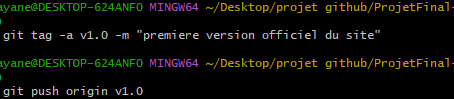
\includegraphics[width=0.7\linewidth]{tag v1.0.png}
    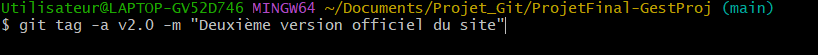
\includegraphics[width=0.7\linewidth]{tag v2.0.png}
    \caption{Captures d'écrans montrant le premier et second tag}
    \label{fig:tag-vrs}
\end{figure}
%%%%%%%%%%%%%%%%%%%% %%%%%%%%%%%%%%%%%%%% %%%%%%%%%%%%%%%%%%%%
\section*{\color{BurntOrange}[B3] Gestion des propositions de contributions}
Nous avons utilisé les \textit{pull requests} lors de modifications majeures ou lorsque l'on préfère demander l'avis d'autres membres du groupe sur ces modifications avant l'intégration à la branche principale (\ref{fig:pll-rqst}).
\newpage

\begin{figure}[ht]
    \centering
    \includegraphics[width=0.7\linewidth]{Pull-Requests.png}
    \caption{Capture d'écran montrant les différents \textit{pull requests} effectués lors du projet}
    \label{fig:pll-rqst}
\end{figure}

%%%%%%%%%%%%%%%%%%%% %%%%%%%%%%%%%%%%%%%% %%%%%%%%%%%%%%%%%%%%

\section*{\color{BurntOrange}[B4] Intégration de site web}

Lien du GitHub Pages : \url{https://gestprojtd3-harm.github.io/ProjetFinal-GestProj/}

%%%%%%%%%%%%%%%%%%%% %%%%%%%%%%%%%%%%%%%% %%%%%%%%%%%%%%%%%%%%

\section*{\color{BrickRed}[C1] Répartition de tâches et milestone}
Nous nous sommes essayés à l'utilisation de \textit{issues} et \textit{milestones}. Cela permet de faire comme des mini-missions temporaires (\ref{fig:issues}) qui peuvent rentrer dans des objectifs plus ou moins globaux (\ref{fig:milestone}).
\begin{figure}[ht]
    \centering
    \includegraphics[width=0.7\linewidth]{OpenIssues.png}
    \includegraphics[width=0.7\linewidth]{ClosedIssues.png}
    \caption{\textit{Issues} ouvertes et fermées}
    \label{fig:issues}
\end{figure}
\begin{figure}[ht]
    \centering
    \includegraphics[width=0.7\linewidth]{ClosedMilestones.png}
    \caption{\textit{Milestone} fermé}
    \label{fig:milestone}
\end{figure}
%%%%%%%%%%%%%%%%%%%% %%%%%%%%%%%%%%%%%%%% %%%%%%%%%%%%%%%%%%%%

\section*{\color{BrickRed}[C2] Intégration continue}

L'intégration continue dans GitHub correspond à une automatisation du travail de vérification après un \textit{push}, qui a pour but de vérifier si le code fonctionne correctement et la qualité de ce dernier, dans notre cas à chaque modification du document HTML/CSS/JS le site web est redéployé par GitHub, seulement après vérification du code par l'automate.
\begin{figure}[ht]
    \centering
    \includegraphics[width=0.7\linewidth]{IntégrationContinue.png}
    \caption{L'ensemble des processus d'intégration continue}
    \label{fig:worflows}
\end{figure}
%%%%%%%%%%%%%%%%%%%% %%%%%%%%%%%%%%%%%%%% %%%%%%%%%%%%%%%%%%%%

\section*{\color{BrickRed}[C3] Gestion de submodule}
Les submodules permettent d'intégrer un autre dépôt Git au sein du projet, le submodule que nous avons choisi nous aide à ajouter des animations CSS à l'HTML à l'aide de classes prédéfinies dans le "sous-module".\\
On utilisera la commande suivante pour intégrer le dépôt à partir de son URL :

\begin{center}
    \textbf{git submodule add https://github.com/animate-css/animate.css}
    \\
    \textbf{git add .gitmodules libs/animate.css}
\end{center}

\begin{figure}[ht]
    \centering
    \includegraphics[width=0.7\linewidth]{ajout sub module .png}
    \includegraphics[width=0.7\linewidth]{ajouter sub.png}
    \caption{Intégration d'un sous-module au projet}
    \label{fig:submodule}
\end{figure}

%%%%%%%%%%%%%%%%%%%% %%%%%%%%%%%%%%%%%%%% %%%%%%%%%%%%%%%%%%%%

%\section*{\color{BrickRed}[C4] Gestion par l'outil \textit{Projet} de \textit{GitHub}}

%%%%%%%%%%%%%%%%%%%% %%%%%%%%%%%%%%%%%%%% %%%%%%%%%%%%%%%%%%%%
\section*{Conclusion}

Ce projet nous a permis d'appliquer sur un cas concret les notions vues en cours et abordées en travaux dirigés. Ceci nous a permis de tester une grande partie des fonctionnalités de Git sur GitHub. Nous n'utilisions pas l'ensemble de ces fonctionnalités dans nos anciens projets et certaines nous étaient inconnues (gestion de sous-modules...). Ceci nous a donc permis de nous familiariser avec, dans un cadre approprié, ce que nous n'aurions pu faire dans le cadre d'un projet classique ou du moins ce qui ne nous serait pas venu en tête.

%%%%%%%%%%%%%%%%%%%% %%%%%%%%%%%%%%%%%%%% %%%%%%%%%%%%%%%%%%%%

\end{document}